%% Paper D: claim-registry case study, for Tecnologia en Marcha (special issue on
%% Artificial Intelligence, deadline 2026-10-15). See docs/reports/paper_d/README.md.
%%
%% The journal takes a Microsoft Word file: letter paper, one column, Times 12 pt,
%% 1.5 line spacing, 5-15 pages, IEEE references, abstracts and keywords in English
%% and Spanish. This LaTeX source is set to the same page so the PDF predicts the
%% Word length; scripts/pubs/build_paper_d.py renders the PDF and the .docx.
%%
%% Review is double-blind. The default build omits author identity; the full build
%% (author block, repository URL) is made by defining \fullversion before this file.
\documentclass[12pt,letterpaper]{article}
\usepackage[margin=25mm]{geometry}
\usepackage{fontspec}
\setmainfont{texgyretermes}[Extension=.otf, UprightFont=*-regular, BoldFont=*-bold,
  ItalicFont=*-italic, BoldItalicFont=*-bolditalic]
\usepackage{setspace}
\onehalfspacing
\usepackage{amsmath}
\usepackage{graphicx}
\usepackage{booktabs}
\usepackage{array}
\usepackage[hidelinks]{hyperref}
\usepackage{cite}
\setlength{\emergencystretch}{3em}

\newif\iffull
\ifdefined\fullversion \fulltrue \else \fullfalse \fi

\begin{document}

\begin{center}
{\large\bfseries Verifiable result traceability in AI research: a claim registry that links
published numbers to their artifacts\par}
\medskip
{\large\bfseries Trazabilidad verificable de resultados en la investigaci\'on en IA: un
registro de afirmaciones que vincula los n\'umeros publicados con sus artefactos\par}
\medskip
\iffull
Jonathan Herrera-V\'asquez\\
Computer scientist. Department of Computer Science, Universidad Americana de Europa
(UNADE), Canc\'un, Quintana Roo, Mexico.\\
jonnabio@gmail.com \quad ORCID: [ORCID]
\else
\textit{Author information omitted for double-blind review.}
\fi
\end{center}

\section*{Abstract}
Numbers in artificial intelligence (AI) research papers are usually copied by hand from
analysis outputs into manuscripts, and when one study feeds a thesis, several papers and
a book chapter, the same number is restated many times. Nothing then checks that each
printed value still matches its source. This paper presents a claim registry, a single
file that records each reported number with a resolver that re-derives it from committed
artifacts and with every place where it is printed, and a verifier that fails the build
on any mismatch, unregistered number or reuse of an unpublished result. We report a case
study of its use in a doctoral research program on explainable AI. At a pinned commit
the registry held 321 claims checked at 487 sites in four documents. We coded 58 defects
recorded by audits, peer-style reviews and root-cause analyses between August and
September 2026. Of the 30 defects that concerned a printed number, the current checks
catch 16 and partly catch 13; of the 28 that concerned claim scope, coherence or
reporting, they catch 3. The continuous-integration workflow failed every one of its
first 37 runs, which shows that a check that never passes protects nothing. Mechanical
verification removes numeric drift as a class of error but leaves overclaiming to human
review.

\noindent\textbf{Keywords:} reproducibility; research software; artificial intelligence;
continuous integration; scientific integrity; explainable AI.

\section*{Resumen}
En la investigaci\'on en inteligencia artificial (IA), los n\'umeros de los art\'iculos
suelen copiarse a mano desde los resultados del an\'alisis hasta los manuscritos, y cuando
un mismo estudio alimenta una tesis, varios art\'iculos y un cap\'itulo de libro, cada
n\'umero se repite muchas veces. Nada verifica entonces que cada valor impreso siga
coincidiendo con su fuente. Este art\'iculo presenta un registro de afirmaciones: un
\'unico archivo que asocia cada n\'umero publicado con un resolvedor que lo recalcula a
partir de artefactos versionados y con cada lugar donde se imprime, junto con un
verificador que detiene la compilaci\'on ante cualquier discrepancia, n\'umero no
registrado o reutilizaci\'on de un resultado no publicado. Se reporta un estudio de caso
de su uso en un programa doctoral sobre IA explicable. En una versi\'on fijada, el
registro conten\'ia 321 afirmaciones verificadas en 487 lugares de cuatro documentos. Se
codificaron 58 defectos registrados por auditor\'ias, revisiones y an\'alisis de causa
ra\'iz entre agosto y septiembre de 2026. De los 30 defectos relativos a un n\'umero
impreso, las verificaciones actuales detectan 16 y detectan parcialmente 13; de los 28
relativos al alcance de las afirmaciones, la coherencia o el reporte, detectan 3. El flujo
de integraci\'on continua fall\'o en sus primeras 37 ejecuciones, lo que muestra que una
verificaci\'on que nunca pasa no protege nada. La verificaci\'on mec\'anica elimina la
deriva num\'erica como clase de error, pero deja la sobreafirmaci\'on a la revisi\'on
humana.

\noindent\textbf{Palabras clave:} reproducibilidad; software de investigaci\'on;
inteligencia artificial; integraci\'on continua; integridad cient\'ifica; IA explicable.

\section{Introduction}

Concern about the reproducibility of computational research is long-standing
\cite{peng2011,sandve2013,stodden2016}, and it has reached artificial intelligence (AI)
in particular \cite{hutson2018,gundersen2018,henderson2018}. Surveys of researchers report
that most have failed to reproduce another group's result \cite{baker2016}; analyses of
machine-learning papers find that undocumented choices and data leakage can change
conclusions \cite{kapoor2023,lipton2019}. Responses have focused on what is released with
a paper: code, data and checklists \cite{pineau2021,heil2021}, data that are findable and
reusable \cite{wilkinson2016}, and notebooks that can be rerun \cite{rule2019,pimentel2019}.

A smaller literature addresses a different failure: the number printed in the paper is
not the number the analysis produced. In psychology, automated checks of reported test
statistics found inconsistencies in about half of the papers examined
\cite{nuijten2016}, and arithmetic checks of reported means exposed further anomalies
\cite{brown2017}. Literate programming and dynamic documents prevent this failure at its
source by generating text and results together \cite{knuth1984,leisch2002,gentleman2007}.

Dynamic documents fit a single report. They fit less well a research program in which one
set of experiments feeds a thesis, several journal manuscripts and a book chapter, each
written by hand in a different format and revised over months. In that setting a number is
restated in many places; a correction made in one document does not reach the others; a
value retired by an audit can reappear in a figure; and a result already published in one
venue can be printed again in a submission to another. None of these is a failure of code
release, so the reproducibility tools above do not detect it.

This paper describes a lightweight mechanism for that setting, a claim registry with an
automated verifier, and evaluates it in a case study. Its contributions are: (i) the design
of the registry and its checks; (ii) an incident catalogue of 58 defects found in one
doctoral program, coded by type and by whether the checks now detect them; and (iii)
evidence on which kinds of error mechanical verification can and cannot remove.

\section{Materials and methods}

\subsection{Research setting}

The case is a doctoral research program on the evaluation of explainable AI methods for
tabular classifiers. Its experiments write per-run result files and statistical exports to
a git repository. Four documents report the results: a thesis (Quarto), a published
journal article and a journal manuscript under review (both \LaTeX), and a book chapter
(Markdown). The same quantities, such as effect sizes, means and run counts, appear in
several of them.

\subsection{The claim registry}

The registry is one TOML file under version control. Its main entry is a \emph{claim}
(Fig.~\ref{fig:architecture}). A claim records an identifier, a \emph{source}
expression, the value as printed, a tolerance, and a list of \emph{sites}. The source
names a resolver, a small function that recomputes the value from committed artifacts.
Each site gives a manuscript file and the literal text that prints the value there.
Let a claim $c$ have registered value $v_c$, tolerance $\tau_c$, resolver $r_c$ and sites
$S_c$. Given the committed artifacts $A$, the claim passes when
\begin{equation}
\lvert r_c(A) - v_c \rvert \le \tau_c
\quad\text{and}\quad
\forall s \in S_c:\ \mathrm{text}(s) \subseteq \mathrm{file}(s).
\label{eq:claim}
\end{equation}
The first condition catches a result that changed after the text was written; the second
catches a manuscript that changed without its result.

Four further entry types close gaps that per-claim checks leave open. A \emph{retired}
entry records a value that an audit removed; the verifier fails if that text reappears in
any manuscript. An \emph{unbacked} entry records a printed number that cannot be
re-derived, with the reason, so that the gap is disclosed rather than hidden.
\emph{Coverage} lists manuscript files that must be fully registered: every numeric
literal $\ell$ found in a covered file $F$ must belong to
\begin{equation}
L(F) \subseteq L_{\text{reg}} \cup L_{\text{ret}} \cup L_{\text{unb}} \cup L_{\text{str}},
\label{eq:coverage}
\end{equation}
the registered, retired, unbacked and declared structural literals (settings,
thresholds, layout values). An unregistered number is therefore a failure, not a silence.
\emph{Exclusivity} lists files that must not print any result registered for an
unpublished manuscript, unless the same result is already published elsewhere.

\subsection{Complementary checks}

Five checks run beside the registry. Abstracts and keywords are generated from one source
file into each manuscript, and a synchronisation check confirms that every manuscript
includes them and that no generated file contains a control character. A shared-literal
scan compares every decimal number in the manuscript under review with those in the
published article, independently of the registry, to detect results reported twice.
Source files reconstructed after a data loss are pinned by hash. The verifier is run from
a fresh clone, because a file present on the author's disk but not tracked by git passes
locally and fails for everyone else. All checks run in continuous integration (CI) on
every push.

\subsection{Implementation}

The verifier and the resolvers are plain Python with no dependency beyond the standard
library and the libraries the analysis already uses. At the pinned commit the verifier had
276 non-blank lines, the resolvers 582, and the registry file 3,076. A verification run
reads the registry, calls every resolver, scans every manuscript listed in a claim, in
coverage or in exclusivity, and prints either one summary line or the list of failures
with the file and line of each. A failure blocks the merge of the change that caused it,
so a manuscript cannot be updated past a number that no longer matches. Adding a number to
a manuscript therefore takes three steps: choose or write the resolver that re-derives it
at the aggregation the text states, add the claim with its site, and print the number.

\subsection{Case-study measurements}

\textit{Registry composition and growth.} The registry was read from git at a pinned
commit, the state after the last refactor of the manuscript under review, and at each of
the commits that changed it since its creation, to count claims, sites and the other entry
types.

\textit{Incident catalogue.} We collected every defect recorded in the program's quality
records between 11 August and 28 September 2026: one cross-document alignment audit,
three peer-style rigor reviews, a coverage triage, a remediation plan, three root-cause
analyses and one chapter synchronisation report. Each entry was coded on four variables: whether it
concerns a printed number; its class (Fig.~\ref{fig:classes}); how it was found (manual
audit or review, building the registry, a coverage sweep, a fresh-clone run, or reading
the rendered output); and whether the current checks would detect it if it were
reintroduced (yes; partly, when the value is checked but its label, aggregation or
context is not; or no). Findings carried forward unchanged from an earlier review, and
findings that are not defects in a document, were excluded. The author coded the
catalogue with AI assistance and checked every entry (see Acknowledgments).

\textit{CI history.} The run history of the CI workflow was exported from the repository
host and summarised by outcome.

All measurements are scripts that read committed files; their outputs are themselves
registered claims of this paper.

\section{Results}

\subsection{Registry composition}

At the pinned commit the registry held 321 claims checked at 487 sites in four documents
(Table~\ref{tab:registry}). 85 claims were printed in more than one document; these are
the values most exposed to cross-document drift. Fifty distinct resolver kinds re-derive
the values. The registry grew from 44 claims at 93 sites when it was created to its
current size over 39 commits (Fig.~\ref{fig:growth}), mostly in two bursts that followed
audits.

\begin{table}[ht]
\centering
\caption{Composition of the claim registry at the pinned commit.}
\label{tab:registry}
\begin{tabular}{lr}
\toprule
Entry & Count \\
\midrule
Claims (re-derived values) & 321 \\
\quad sites in the thesis & 286 \\
\quad sites in the manuscript under review & 146 \\
\quad sites in the book chapter & 30 \\
\quad sites in the published article & 18 \\
Retired values & 27 \\
Unbacked values & 10 \\
Declared structural literals & 69 \\
Files under coverage & 19 \\
Files under exclusivity & 13 \\
\bottomrule
\end{tabular}
\end{table}

\begin{figure}[ht]
\centering
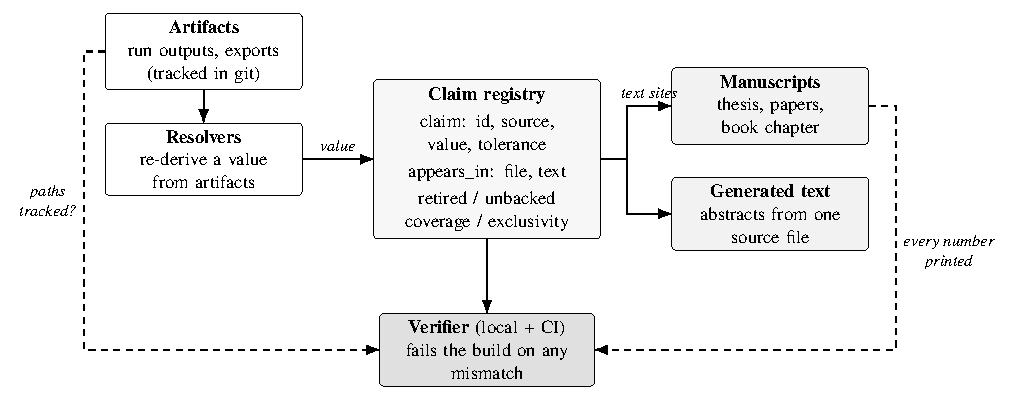
\includegraphics[width=0.8\linewidth]{figures/fig1_architecture}
\caption{The verification loop. A resolver re-derives each registered value from tracked
artifacts; the verifier compares it with the registered value and with the text at every
manuscript site, and checks that cited artifacts are tracked.}
\label{fig:architecture}
\end{figure}

\begin{figure}[ht]
\centering
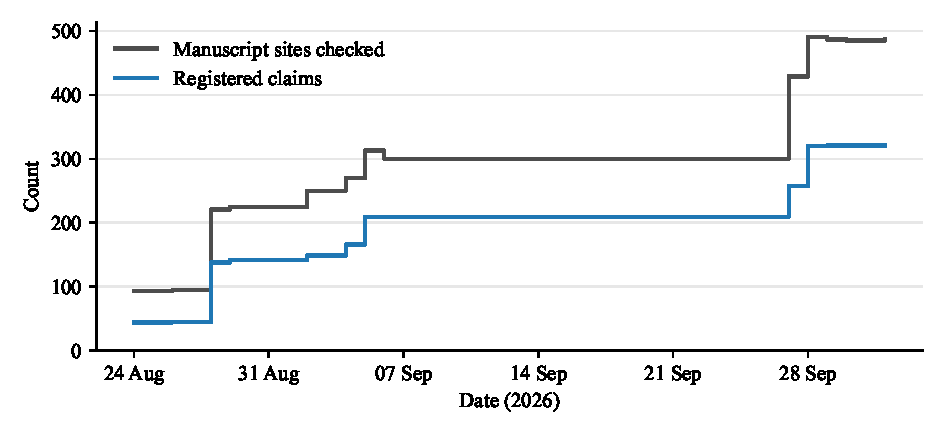
\includegraphics[width=0.8\linewidth]{figures/fig2_registry_growth}
\caption{Growth of the registry: claims and checked manuscript sites at each day on which
the registry changed.}
\label{fig:growth}
\end{figure}

\subsection{Incident catalogue}

The quality records yielded 65 entries, of which 58 were distinct defects in a document;
22 were rated major. Thirty concerned a printed number and 28 did not.
Fig.~\ref{fig:classes} shows the defects by class and by whether the current checks detect
them.

For numeric defects the checks are effective. Of the 30, 16 would be detected and 13
would be partly detected; one would not, a traceability table that cited an existing but
wrong artifact, which passes because the verifier checks that a cited file exists, not
that it is the right file. The partly detected defects share a pattern: the value is
right, and what is wrong is the text around it. Examples are a correct gap attributed to
the wrong model, run-level means labelled as block-level means, and a sample size in a
caption that belongs to a different statistic.

For non-numeric defects the picture reverses. Of the 28, the checks detect 3, all of them
mechanical failures: an escape sequence that corrupted a generated abstract, a
supplementary file missing from an upload bundle, and a verification input that existed on
one machine only. The other 25 are claims stated more broadly than the evidence,
internal contradictions between sections, and reporting slips. The largest single class,
claim scope, is almost invisible to them: 12 of its 13 defects are not detected.

Most defects, 47 of the 58, were found by people reading: the audit and the reviews.
Eight defects were found by the tooling itself, while the registry was being built or
extended: registering a value forced a comparison with its artifact, and the coverage
sweep surfaced numbers that nobody had registered. The remaining three were found by
reading the rendered output, which is where a broken cross-reference or a corrupted
generated abstract becomes visible. Table~\ref{tab:examples} gives one example per class
and the check, if any, that now responds to it.

\begin{table}[ht]
\centering
\caption{Example defects from the catalogue and the response of the current checks.}
\label{tab:examples}
\small
\begin{tabular}{>{\raggedright\arraybackslash}p{33mm}>{\raggedright\arraybackslash}p{63mm}>{\raggedright\arraybackslash}p{52mm}}
\toprule
Class & Example & Current response \\
\midrule
Value differs from artifact & A chapter printed draft figures that matched no artifact &
Detected: the site text no longer matches the re-derived value \\
Cross-document inconsistency & Two manuscripts printed different values for one
experimental cell & Detected: one claim carries the sites of both \\
Wrong label or aggregation & A correct gap attributed to the wrong model & Partly: the
value is checked, the label is not \\
Value without an artifact & Two tables printed different values for one reference
condition & Partly: the number must be declared unbacked, with a reason \\
Artifact provenance & Cited result files present on disk but not tracked by git &
Detected: the fresh-clone run fails \\
Prior-publication overlap & Results of a published article printed again in a
submission & Detected: the shared-literal scan fails \\
Rendering defect & An escape sequence corrupted a generated abstract & Detected: the
synchronisation check fails \\
Claim scope & An ordering claimed for a model family that holds for one member only &
Not detected \\
\bottomrule
\end{tabular}
\end{table}

\begin{figure}[ht]
\centering
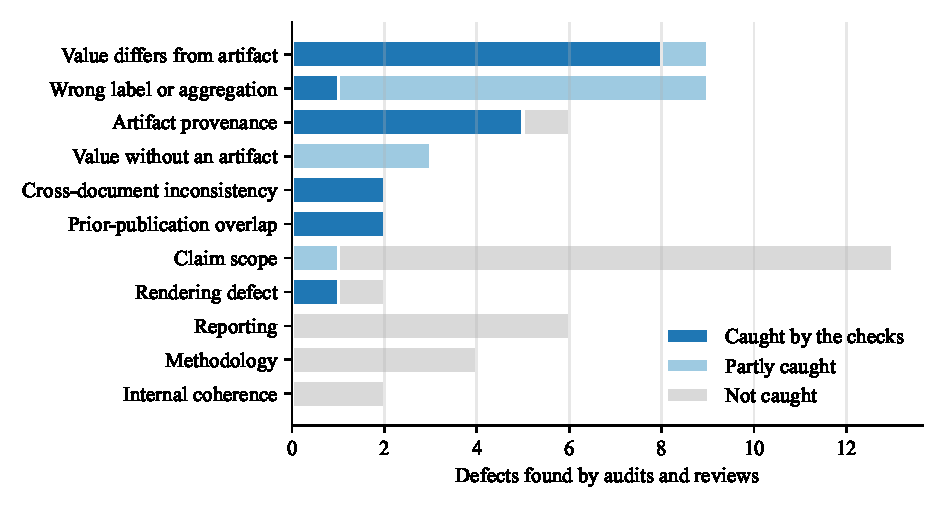
\includegraphics[width=0.8\linewidth]{figures/fig3_incident_classes}
\caption{The 58 defects by class and by whether the current checks detect them.}
\label{fig:classes}
\end{figure}

\subsection{Continuous-integration history}

The CI workflow ran 80 times. Its first 37 runs all failed. The causes recorded when
the workflow was investigated were in its environment (an input file that was not tracked
and a generated file that changed on every build), not in the manuscripts. For five months
the check was red for reasons unrelated to what it was meant to protect, so its failures
carried no information. After those causes were fixed, all 43 runs passed.

\section{Discussion}

The case supports a narrow conclusion. A registry that binds each printed number to its
artifact and to every place it appears removes numeric drift as a class of error: a
stale value, a retired value that comes back, a number that differs between two
documents, an unregistered number and a result reported twice all fail the build. These
were the defects that the August audit had found by reading.

Three lessons concern what the mechanism does not do. First, checking a value is not
checking its meaning. The partly detected defects show that a correct number attached to
the wrong label passes; binding the label or the aggregation to the site text, rather
than the number alone, would close part of this gap. Second, about half of all defects
were about claims, not numbers. Scope, coherence and reporting need human review, and the
registry helps only indirectly, by freeing reviewers from re-deriving numbers. Third, a
check must be kept green to be useful: a workflow that fails for unrelated reasons trains
its users to ignore it.

\textit{Limitations.} This is one program, coded by its author, who also built the
tooling; the coding of ``detected now'' was not checked by a second rater and may favour
the tool. The catalogue covers only the defects that audits and reviews recorded, so the
rate of undetected defects is unknown. The registry adds work: every new number must be
registered with a resolver before it is printed.

\textit{Relation to existing tools.} Automated consistency checks of reported statistics
\cite{nuijten2016,brown2017} test whether numbers in a published paper agree with each
other; they need no access to the data, but they cannot tell whether a value is the one
the analysis produced. Dynamic documents \cite{leisch2002,gentleman2007} guarantee that
correspondence within one document, at the price of writing the document inside the
analysis environment. The registry sits between the two: manuscripts stay in whatever
format each venue requires and are written by hand, and the correspondence with the
artifacts is checked from outside. It also checks a property neither approach addresses,
that a result is not reported twice across venues.

\textit{Recommendations.} For research programs that report the same results in several
documents: register each reported number once, with every site; record retired values
so they cannot return; treat an unregistered number in a finished manuscript as an error;
check prior publication by comparing numbers, not only text; run the checks from a fresh
clone and in CI; and keep human review for claims.

\section{Conclusions}

A claim registry is a small, practical addition to the reproducibility toolkit for AI
research. In the case studied it re-derived 321 reported values at 487 sites and would now
detect almost all of the numeric defects that manual audits had found. It does not detect
overclaiming, which was as common as numeric error. Release of code and data shows that a
result can be reproduced; a registry shows that the paper reports the result that was
produced.

\section*{Data availability}
\iffull
The registry, the verifier, the measurement scripts and the incident catalogue are in
the public repository \url{https://github.com/jonnabio/xai-eval-framework}, archived at
\url{https://doi.org/10.5281/zenodo.23111684}.
\else
The registry, the verifier, the measurement scripts and the incident catalogue are in a
public repository and a versioned archive whose addresses are withheld for double-blind
review.
\fi

\section*{Acknowledgments}
The author conceived, designed and directed this work. Generative AI tools (Anthropic
Claude) were used as assistants under the author's direction for programming support,
first-pass coding of the incident catalogue (checked and approved by the author), the
search for related literature (every reference was verified against its DOI record and
approved by the author), and language editing. The author takes full responsibility for
the content.

\bibliographystyle{IEEEtran}
\bibliography{references}

\end{document}
